\chapter{Einleitung}
\label{cha:einleitung}

\section{Motivation}
Die Cloud (Cloud Computing) weist einen immer größer werdenden Stellenwert in der Wirtschaft auf. Durch die zahlreichen
Möglichkeiten, die sich durch die Nutzung einer Cloud ergeben, beschäftigen sich immer mehr Unternehmen mit diesem Thema.

Ein großes Problem, vor allem deutscher Unternehmen, ist der Datenschutz. Sensible Daten dürfen nicht in die Cloud geladen
und sollen weiterhin eigenständig verwaltet und geschützt werden. Viele Unternehmen sind auf ihre bisherige Infrastruktur
angewiesen und werden diese nicht komplett in die Cloud migrieren. Dies kann rechtliche, firmenpolitische oder strategische
Gründe haben.

Trotzdem  bietet die Cloud zahlreiche Funktionen, welche Unternehmen in ihre bestehende Infrastruktur oder Anwendungen
einbinden möchten, um diese zu optimieren (siehe \cite{online_einleitung_datensicherheit}).

Andererseits dauert es Mitarbeitern in den entsprechenden Entwicklungsabteilungen oftmals zu lange, bis der Systemadministrator
die geforderten Programme und Benutzer eingerichtet hat. Oft steht die erforderliche Hard- oder Software nicht zur
Verfügung und muss erst beschafft werden oder es existieren interne Prozesse, welche die Beschaffung oder die Einrichtung
verlangsamen oder gar verhindern. Somit ist keine schnelle und agile Entwicklung möglich.

Um dem entgegenzuwirken greifen Entwickler, um schnell einen Prototypen bauen zu können, oft auf eine vorhandene
Cloud-Infrastruktur zurück. Diese ist schnell einsatzbereit und verursacht keine großen finanziellen Belastungen für das
Unternehmen (siehe \cite{online_einleitung_cloud} und \cite{online_grundlagen_cloudusage}).

Außerdem können durch die Cloud Kosten gespart werden, welche ansonsten in die Vorhaltung von Ressourcen geflossen sind,
um auftretende Engpässe zu umgehen. Desweiteren kann in der Cloud Software genutzt werden, die im Unternehmen gar nicht
bereit steht oder das Know-How darüber nicht existiert.

Problematisch wird es, wenn ein gebauter Prototyp die Gremien überzeugen konnte und nun live gehen soll. Meist arbeiten
Prototypen mit beispielhaften Daten, welche ab sofort durch reale Daten aus dem Rechenzentrum ersetzt werden müssen. Die
Migration auf die Hard- und Software im Rechenzentrum ist allerdings nicht immer ohne Aufwand möglich. Außerdem funktioniert
die Anwendung schon und soll nicht unnötig ein zweites Mal entwickelt werden.

Auch gibt es auf dem Mainframe Anwendungen oder Datenbestände in Datenbanken, welche einer Cloud-Anwendung als Service
bereit gestellt werden sollen, um zum Beispiel Smartphone-Apps  für die Mitarbeiter bereit zu stellen.

Die Gründe für die Hybrid-Cloud-Architektur sind in Abbildung \ref{fig:plakat} illustriert.

Ziel dieser Arbeit ist es, eine Architektur zu entwickeln, die eine in der Cloud gebaute Anwendung sicher in die bestehende
Infrastruktur einbinden kann.

\begin{figure}[h]
  \centering
    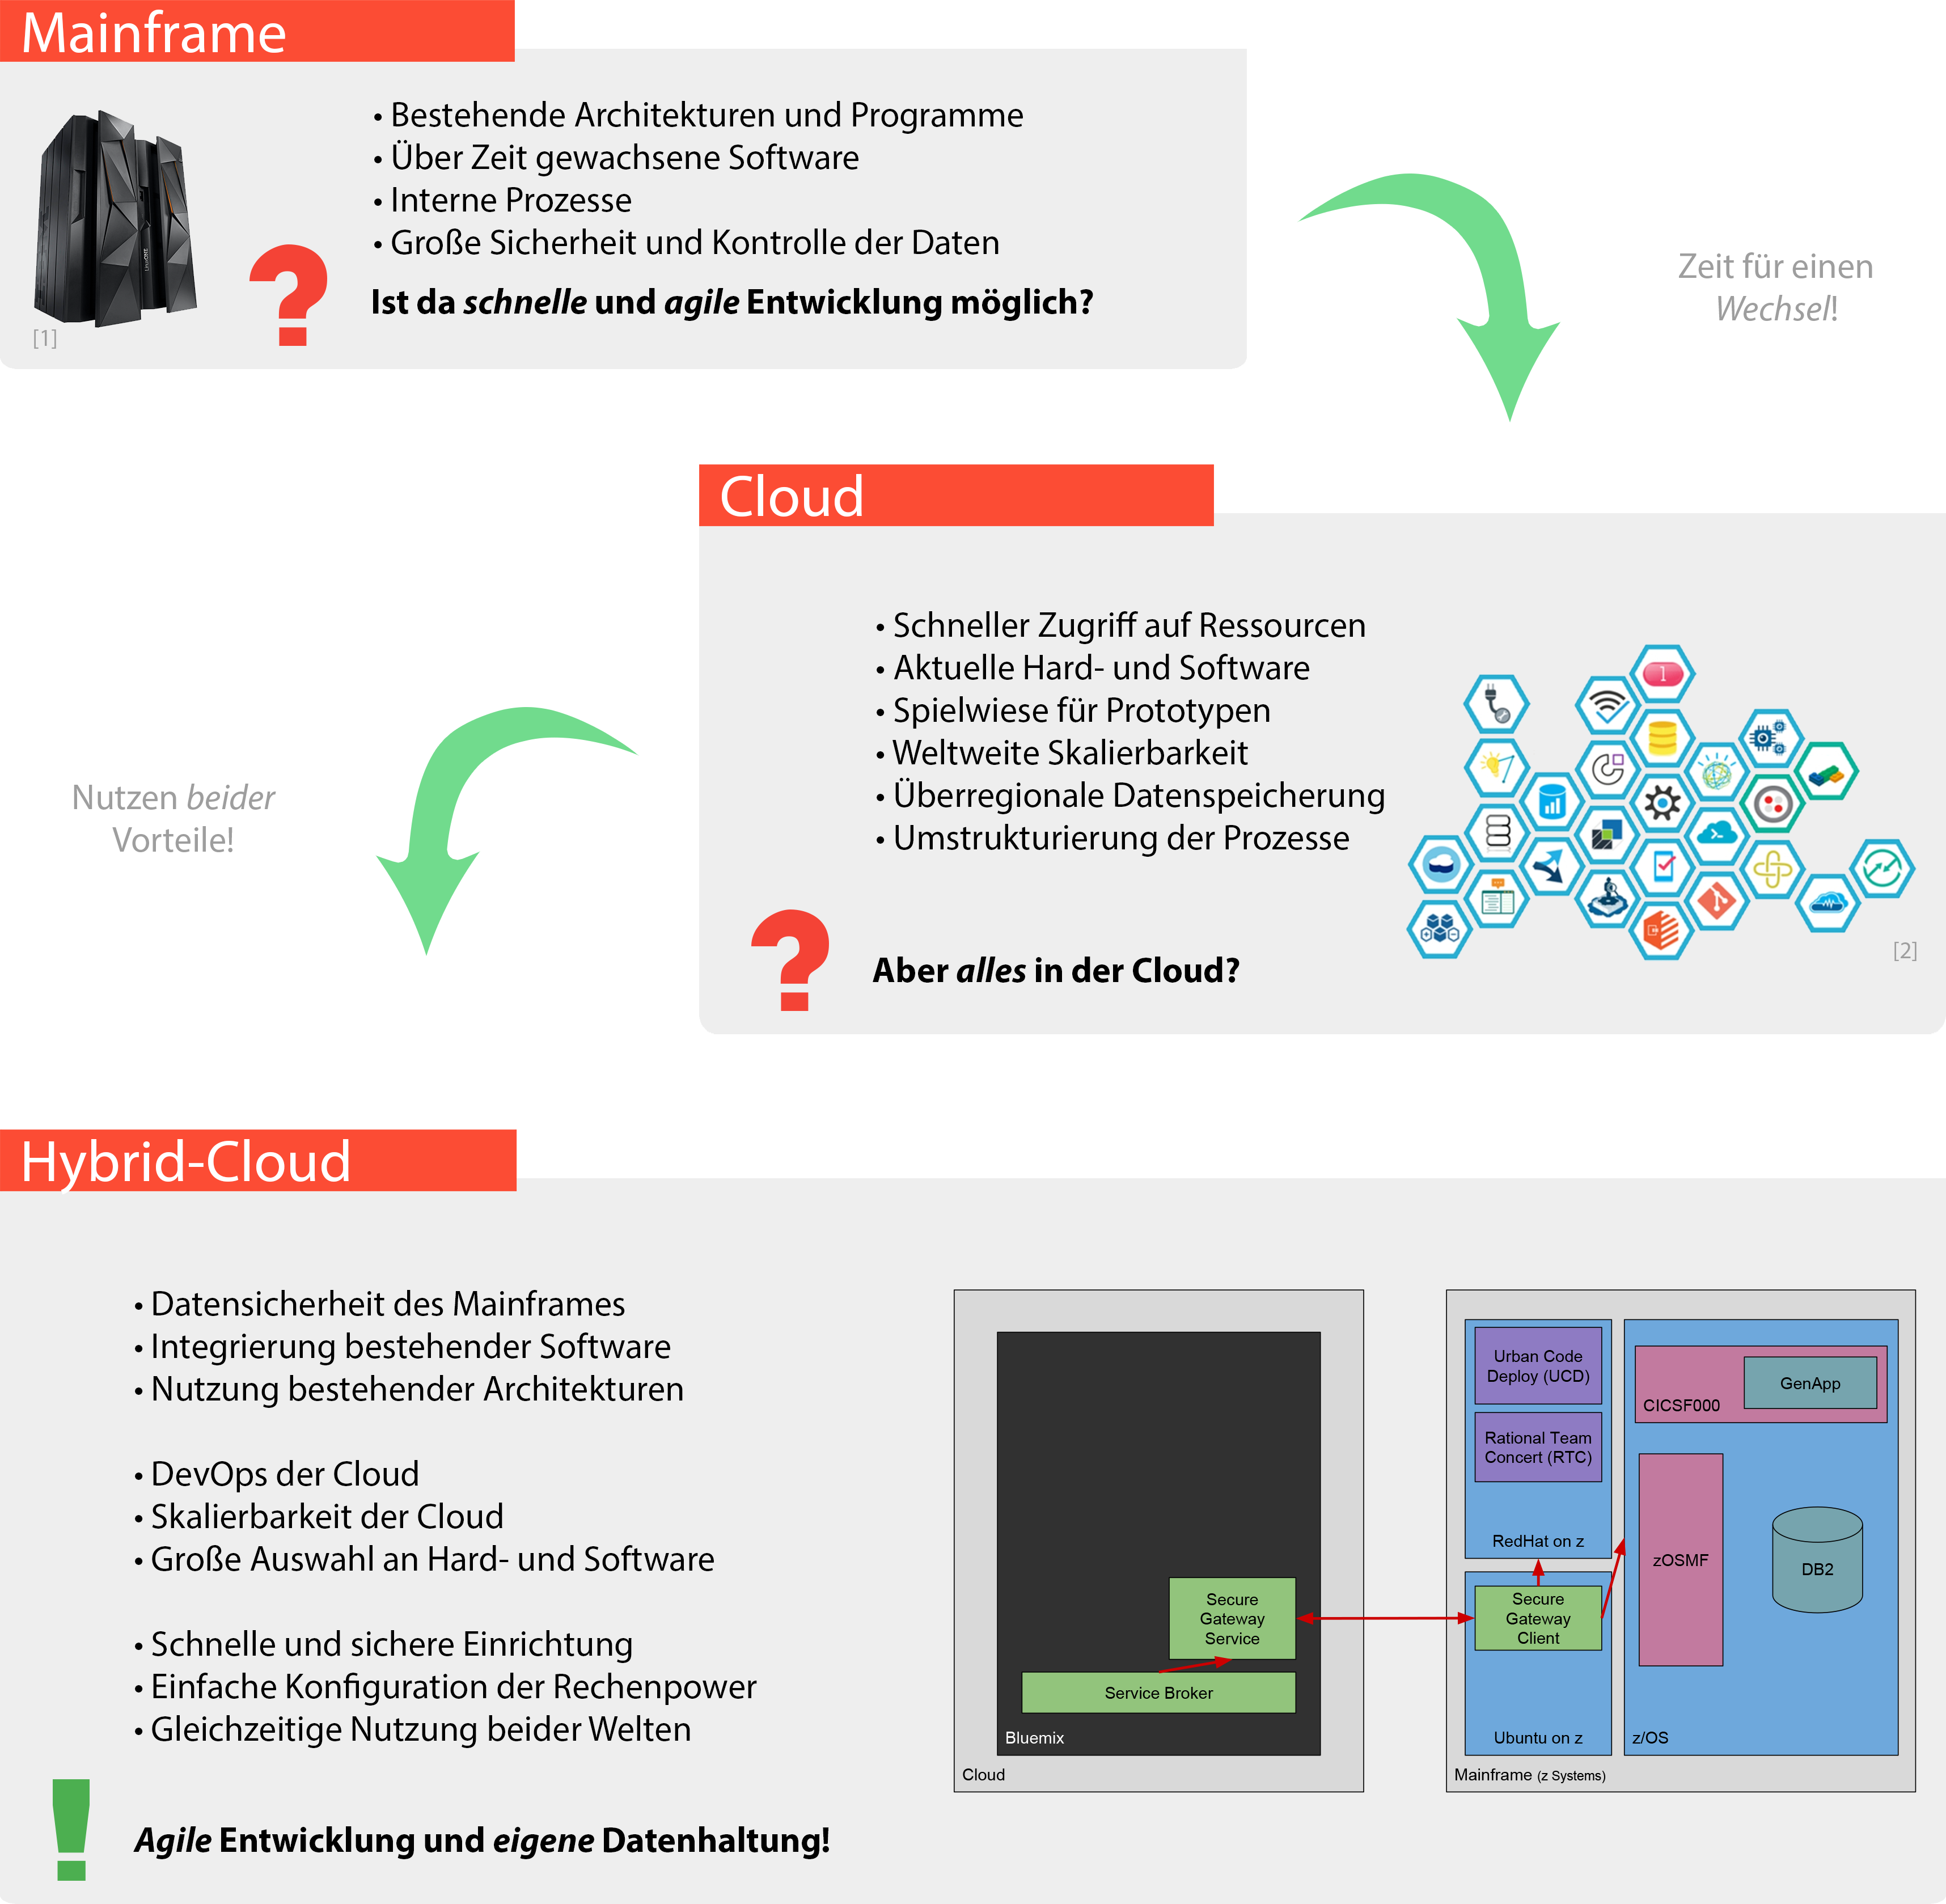
\includegraphics[scale=0.104]{images/kapitel_1/plakat.png}
  \caption{Entstehung der Hybrid-Cloud}
  \label{fig:plakat}
\end{figure}

\newpage

\section{Aufgabenstellung}
Das Kapitel soll eine kleine Übersicht über die Themen geben, welche in der Arbeit behandelt werden. Die Arbeit ist
in drei Themenbereiche unterteilt.

Der erste Teil der Arbeit befasst sich mit der Entwicklung einer Hybrid-Cloud-"-Architektur, welche die Cloud Infrastruktur
und die lokale Mainframe-Welt verbindet. Ein Unternehmen soll seine aufgebaute Mainframe-Umgebung weiter benutzen, aber
gleichzeitig die Vorteile der Cloud nutzen können.

Dazu zählen unter anderem die agilen Möglichkeiten bei der Entwicklung einer Anwendung (DevOps), höhere Geschwindigkeiten
bei der Freigabe neuer Releases und die einfache Verteilung der Applikationen über die ganze Welt ohne eigene Hardware
vorhalten zu müssen. Außerdem spielt die Skalierbarkeit und die Verfügbarkeit der eigenen Anwendung eine wichtige Rolle,
bei der die Cloud unterstützen kann.

Im zweiten Teil der Arbeit wird eine prototypische Anwendung entwickelt, welche die erstellte Architektur prototypisch
implementiert. Dabei soll die Architektur einer Machbarkeitsstudie unterzogen werden. Die Anwendung besteht aus einer
DB2 Instanz, einer COBOL-"-Runtime, einer COBOL-"-Anwendung, einem Java-"-Backend, einem Web-Frontend und zwei
Smartphone-"-Apps.

Der letzte Teil widmet sich dem Thema Qualitätssicherung in diesem Szenario. Fragen sind zum Beispiel, wie bei immer
schneller werdenden Releasezyklen die richtige Qualität der Anwendung gewahrt werden kann. Außerdem wird gezeigt, wie
die prototypische Anwendung aus dem zweiten Teil der Arbeit getestet werden kann.

Zum Schluss folgt ein Ausblick mit Anregungen und Ergänzungen sowohl für die Weiterentwicklung der Hybrid-Cloud-Architektur
als auch für das Web-Frontend und die Smartphone-Apps.

Ziel ist es, einem Unternehmen dabei zu helfen die Vorteile der Cloud und des Mainframes gemeinsam zu nutzen
ohne einen größeren Aufwand zu generieren. Außerdem soll aufgezeigt werden, wie bestehende Anwendungen als Services
für die Cloud bereit gestellt werden können.

\newpage

\section{Aufbau der Arbeit}
Dieses Kapitel dient zur schnellen Orientierung innerhalb der Arbeit und soll detaillierter zeigen, welche Themen in den
jeweiligen Kapiteln angesprochen werden.

\begin{description}

\item[Kapitel 2 (Grundlagen)]\hfill \\
In diesem Kapitel werden die Grundlagen erklärt. Es wird zum Beispiel der Unterschied einer Cloud zu einer Hybrid-Cloud
erläutert, um was es sich bei Bluemix handelt und was ein WebViewer ist.

\item[Kapitel 3 (Hybrid-Cloud-Architektur)]\hfill \\
Im dritten Kapitel wird eine Hybrid-Cloud-Architektur entwickelt und umgesetzt. Dabei werden verschiedene Optionen
für die einzelnen Teilaufgaben analysiert und im Anschluss die genutzten Programme installiert, eingerichtet und erläutert.
Anschließend wird die Architektur implementiert.

\item[Kapitel 4 (Prototypische Anwendung)]\hfill \\
Das vierte Kapitel setzt die Hybrid-Cloud-Architektur voraus und implementiert dazu eine prototypische Anwendung. Diese
besteht aus einem Backend, einem Frontend und zwei Smartphone-Apps. Dabei werden zu Anfang verschiedene Programme und
Services analysiert, um diese im Anschluss zu nutzen.

\item[Kapitel 5 (Qualitätssicherung)]\hfill \\
Dieses Kapitel beschäftigt sich mit dem Thema Qualitätssicherung und wie die Qualität bei immer schneller werdenen
Releasezyklen gewahrt werden kann. Dabei spielen automatische Tests eine wichtige Rolle.

\item[Kapitel 6 (Diskussion)]\hfill \\
Hier werden Themen angesprochen, die für die Verwendung der Hybrid-Cloud-\-Architektur erläutert werden müssen.
Unter anderem welche Rechte Entwickler in Zukunft haben sollen oder welche Use-Cases es für die Architektur gibt.

\item[Kapitel 7 (Ausblick)]\hfill \\
Wie sowohl die entwickelte Hybrid-\-Cloud-\-Architektur als auch die Anwendung erweitert werden können, wird in diesem
Kapitel aufgezeigt. Dabei können neue Cloud-Services hinzugefügt oder auch weitere Funktionen der schon eingesetzten
Services verwendet werden.

\item[Kapitel 8 (Zusammenfassung)]\hfill \\
Das letzte Kapitel enthält eine Zusammenfassung aller vorangegangenen Kapitel und ein Schlusswort.

\end{description}